\documentclass{standalone}
\usepackage{tikz}
\usetikzlibrary{patterns, positioning}


\begin{document}
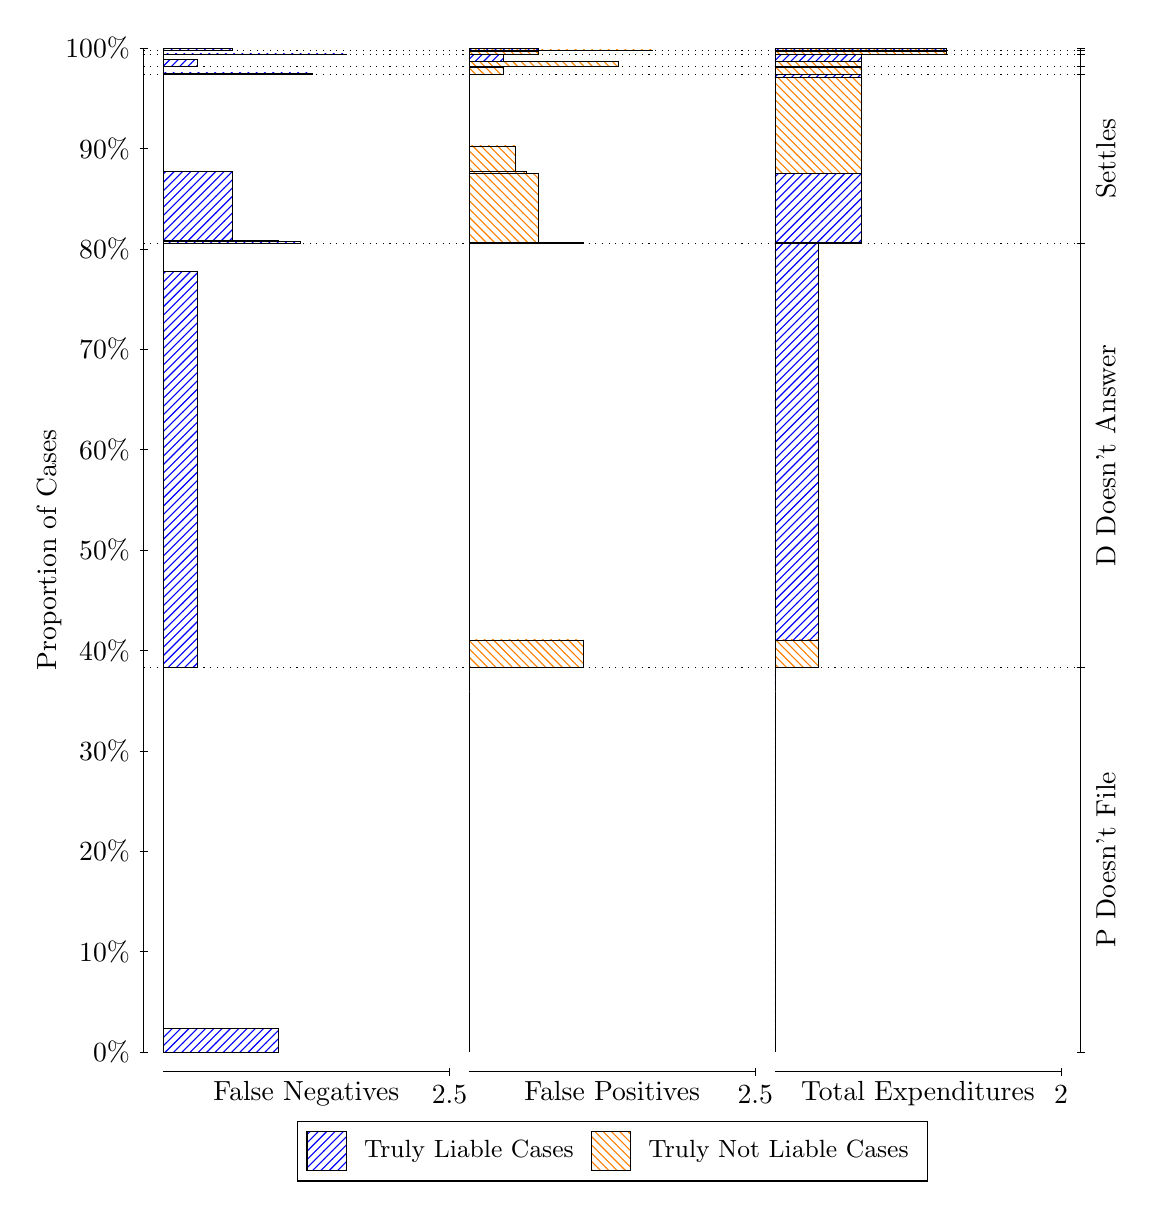
\begin{tikzpicture}
\draw[black, very thin] (1.5,1.75) -- (1.5,14.5);
\node[rotate=90, text=black, anchor=center] at (0.3, 8.125) {Proportion of Cases};
\draw[black, very thin] (1.45,1.75) -- (1.55,1.75);
\node[text=black, anchor=east] at (1.45, 1.75) {0\%};
\draw[black, very thin] (1.45,3.025) -- (1.55,3.025);
\node[text=black, anchor=east] at (1.45, 3.025) {10\%};
\draw[black, very thin] (1.45,4.3) -- (1.55,4.3);
\node[text=black, anchor=east] at (1.45, 4.3) {20\%};
\draw[black, very thin] (1.45,5.575) -- (1.55,5.575);
\node[text=black, anchor=east] at (1.45, 5.575) {30\%};
\draw[black, very thin] (1.45,6.85) -- (1.55,6.85);
\node[text=black, anchor=east] at (1.45, 6.85) {40\%};
\draw[black, very thin] (1.45,8.125) -- (1.55,8.125);
\node[text=black, anchor=east] at (1.45, 8.125) {50\%};
\draw[black, very thin] (1.45,9.4) -- (1.55,9.4);
\node[text=black, anchor=east] at (1.45, 9.4) {60\%};
\draw[black, very thin] (1.45,10.675) -- (1.55,10.675);
\node[text=black, anchor=east] at (1.45, 10.675) {70\%};
\draw[black, very thin] (1.45,11.95) -- (1.55,11.95);
\node[text=black, anchor=east] at (1.45, 11.95) {80\%};
\draw[black, very thin] (1.45,13.225) -- (1.55,13.225);
\node[text=black, anchor=east] at (1.45, 13.225) {90\%};
\draw[black, very thin] (1.45,14.5) -- (1.55,14.5);
\node[text=black, anchor=east] at (1.45, 14.5) {100\%};

\draw[black, very thin] (13.4,1.75) -- (13.4,14.5);
\draw[black, very thin] (13.35,1.75) -- (13.45,1.75);
\node[anchor=west] at (13.35, 1.75) {};
\draw[black, very thin] (13.35,6.6296) -- (13.45,6.6296);
\node[anchor=west] at (13.35, 6.6296) {};
\draw[black, very thin] (13.35,12.02) -- (13.45,12.02);
\node[anchor=west] at (13.35, 12.02) {};
\draw[black, very thin] (13.35,14.169) -- (13.45,14.169);
\node[anchor=west] at (13.35, 14.169) {};
\draw[black, very thin] (13.35,14.268) -- (13.45,14.268);
\node[anchor=west] at (13.35, 14.268) {};
\draw[black, very thin] (13.35,14.42) -- (13.45,14.42);
\node[anchor=west] at (13.35, 14.42) {};
\draw[black, very thin] (13.35,14.47) -- (13.45,14.47);
\node[anchor=west] at (13.35, 14.47) {};
\draw[black, very thin] (13.35,14.5) -- (13.45,14.5);
\node[anchor=west] at (13.35, 14.5) {};

\draw[black, very thin, pattern color=blue, pattern=north east lines] (1.75,1.75) rectangle (3.2033,2.0495);
\draw[black, very thin, pattern color=orange, pattern=north west lines] (1.75,2.0495) rectangle (1.75,6.6296);
\draw[black, very thin, pattern color=blue, pattern=north east lines] (1.75,6.6296) rectangle (2.186,11.665);
\draw[black, very thin, pattern color=orange, pattern=north west lines] (1.75,11.665) rectangle (1.75,12.02);
\draw[black, very thin, pattern color=blue, pattern=north east lines] (1.75,12.02) rectangle (3.494,12.042);
\draw[black, very thin, pattern color=blue, pattern=north east lines] (1.75,12.042) rectangle (3.3487,12.046);
\draw[black, very thin, pattern color=blue, pattern=north east lines] (1.75,12.046) rectangle (3.2033,12.059);
\draw[black, very thin, pattern color=blue, pattern=north east lines] (1.75,12.059) rectangle (2.622,12.93);
\draw[black, very thin, pattern color=orange, pattern=north west lines] (1.75,12.93) rectangle (1.75,14.169);
\draw[black, very thin, pattern color=blue, pattern=north east lines] (1.75,14.169) rectangle (3.6393,14.184);
\draw[black, very thin, pattern color=orange, pattern=north west lines] (1.75,14.184) rectangle (1.75,14.268);
\draw[black, very thin, pattern color=blue, pattern=north east lines] (1.75,14.268) rectangle (2.186,14.355);
\draw[black, very thin, pattern color=orange, pattern=north west lines] (1.75,14.355) rectangle (1.75,14.42);
\draw[black, very thin, pattern color=blue, pattern=north east lines] (1.75,14.42) rectangle (4.0753,14.425);
\draw[black, very thin, pattern color=orange, pattern=north west lines] (1.75,14.425) rectangle (1.75,14.47);
\draw[black, very thin, pattern color=blue, pattern=north east lines] (1.75,14.47) rectangle (2.622,14.493);
\draw[black, very thin, pattern color=orange, pattern=north west lines] (1.75,14.493) rectangle (1.75,14.5);
\draw[black, very thin, pattern color=orange, pattern=north west lines] (5.6333,1.75) rectangle (5.6333,6.3301);
\draw[black, very thin, pattern color=blue, pattern=north east lines] (5.6333,6.3301) rectangle (5.6333,6.6296);
\draw[black, very thin, pattern color=orange, pattern=north west lines] (5.6333,6.6296) rectangle (7.0867,6.9841);
\draw[black, very thin, pattern color=blue, pattern=north east lines] (5.6333,6.9841) rectangle (5.6333,12.02);
\draw[black, very thin, pattern color=orange, pattern=north west lines] (5.6333,12.02) rectangle (7.0867,12.032);
\draw[black, very thin, pattern color=orange, pattern=north west lines] (5.6333,12.032) rectangle (6.5053,12.907);
\draw[black, very thin, pattern color=orange, pattern=north west lines] (5.6333,12.907) rectangle (6.36,12.936);
\draw[black, very thin, pattern color=orange, pattern=north west lines] (5.6333,12.936) rectangle (6.2147,13.258);
\draw[black, very thin, pattern color=blue, pattern=north east lines] (5.6333,13.258) rectangle (5.6333,14.169);
\draw[black, very thin, pattern color=orange, pattern=north west lines] (5.6333,14.169) rectangle (6.0693,14.253);
\draw[black, very thin, pattern color=blue, pattern=north east lines] (5.6333,14.253) rectangle (5.6333,14.268);
\draw[black, very thin, pattern color=orange, pattern=north west lines] (5.6333,14.268) rectangle (7.5227,14.333);
\draw[black, very thin, pattern color=blue, pattern=north east lines] (5.6333,14.333) rectangle (6.0693,14.42);
\draw[black, very thin, pattern color=orange, pattern=north west lines] (5.6333,14.42) rectangle (6.5053,14.465);
\draw[black, very thin, pattern color=blue, pattern=north east lines] (5.6333,14.465) rectangle (5.6333,14.47);
\draw[black, very thin, pattern color=orange, pattern=north west lines] (5.6333,14.47) rectangle (7.9587,14.477);
\draw[black, very thin, pattern color=blue, pattern=north east lines] (5.6333,14.477) rectangle (6.5053,14.5);
\draw[black, very thin, pattern color=orange, pattern=north west lines] (9.5167,1.75) rectangle (9.5167,6.3301);
\draw[black, very thin, pattern color=blue, pattern=north east lines] (9.5167,6.3301) rectangle (9.5167,6.6296);
\draw[black, very thin, pattern color=orange, pattern=north west lines] (9.5167,6.6296) rectangle (10.062,6.9841);
\draw[black, very thin, pattern color=blue, pattern=north east lines] (9.5167,6.9841) rectangle (10.062,12.02);
\draw[black, very thin, pattern color=orange, pattern=north west lines] (9.5167,12.02) rectangle (10.607,12.032);
\draw[black, very thin, pattern color=blue, pattern=north east lines] (9.5167,12.032) rectangle (10.607,12.904);
\draw[black, very thin, pattern color=orange, pattern=north west lines] (9.5167,12.904) rectangle (10.607,14.13);
\draw[black, very thin, pattern color=blue, pattern=north east lines] (9.5167,14.13) rectangle (10.607,14.169);
\draw[black, very thin, pattern color=orange, pattern=north west lines] (9.5167,14.169) rectangle (10.607,14.253);
\draw[black, very thin, pattern color=blue, pattern=north east lines] (9.5167,14.253) rectangle (10.607,14.268);
\draw[black, very thin, pattern color=orange, pattern=north west lines] (9.5167,14.268) rectangle (10.607,14.333);
\draw[black, very thin, pattern color=blue, pattern=north east lines] (9.5167,14.333) rectangle (10.607,14.42);
\draw[black, very thin, pattern color=orange, pattern=north west lines] (9.5167,14.42) rectangle (11.697,14.465);
\draw[black, very thin, pattern color=blue, pattern=north east lines] (9.5167,14.465) rectangle (11.697,14.47);
\draw[black, very thin, pattern color=orange, pattern=north west lines] (9.5167,14.47) rectangle (11.697,14.477);
\draw[black, very thin, pattern color=blue, pattern=north east lines] (9.5167,14.477) rectangle (11.697,14.5);
\draw[black, dotted] (1.5,6.6296) -- (13.4,6.6296);
\draw[black, dotted] (1.5,12.02) -- (13.4,12.02);
\draw[black, dotted] (1.5,14.169) -- (13.4,14.169);
\draw[black, dotted] (1.5,14.268) -- (13.4,14.268);
\draw[black, dotted] (1.5,14.42) -- (13.4,14.42);
\draw[black, dotted] (1.5,14.47) -- (13.4,14.47);
\draw[black, very thin] (1.75,1.5) -- (5.3833,1.5);
\node[text=black, anchor=north] at (3.5667, 1.5) {False Negatives};
\draw[black, very thin] (5.3833,1.45) -- (5.3833,1.55);
\node[text=black, anchor=north] at (5.3833, 1.45) {2.5};

\draw[black, very thin] (5.6333,1.5) -- (9.2667,1.5);
\node[text=black, anchor=north] at (7.45, 1.5) {False Positives};
\draw[black, very thin] (9.2667,1.45) -- (9.2667,1.55);
\node[text=black, anchor=north] at (9.2667, 1.45) {2.5};

\draw[black, very thin] (9.5167,1.5) -- (13.15,1.5);
\node[text=black, anchor=north] at (11.333, 1.5) {Total Expenditures};
\draw[black, very thin] (13.15,1.45) -- (13.15,1.55);
\node[text=black, anchor=north] at (13.15, 1.45) {2};

\node[text=black, centered, rotate=90] at (13.72, 4.1898) {P Doesn't File};
\node[text=black, centered, rotate=90] at (13.72, 9.3246) {D Doesn't Answer};
\node[text=black, centered, rotate=90] at (13.72, 13.094) {Settles};





\draw (7.449999999999999,1.5) node[draw=none] (baseCoordinate) {};
\begin{scope}[align=center]
        \matrix[scale=0.5, draw=black, below=0.5cm of baseCoordinate, nodes={draw}, column sep=0.1cm]{
            \node[rectangle, draw, minimum width=0.5cm, minimum height=0.5cm, pattern color=blue, pattern=north east lines] {}; &
            \node[draw=none, font=\small, text=black] (B) {Truly Liable Cases}; &
            \node[rectangle, draw, minimum width=0.5cm, minimum height=0.5cm, pattern color=orange, pattern=north west lines] {}; &
            \node[draw=none, font=\small, text=black] (B) {Truly Not Liable Cases}; \\
            };
\end{scope}

\end{tikzpicture}
\end{document}